\documentclass[border=4pt]{standalone}
\usepackage{tikz}
\usetikzlibrary{positioning, arrows.meta, calc, fit, backgrounds, decorations.pathmorphing}
\usepackage{amsmath,amssymb}

\begin{document}
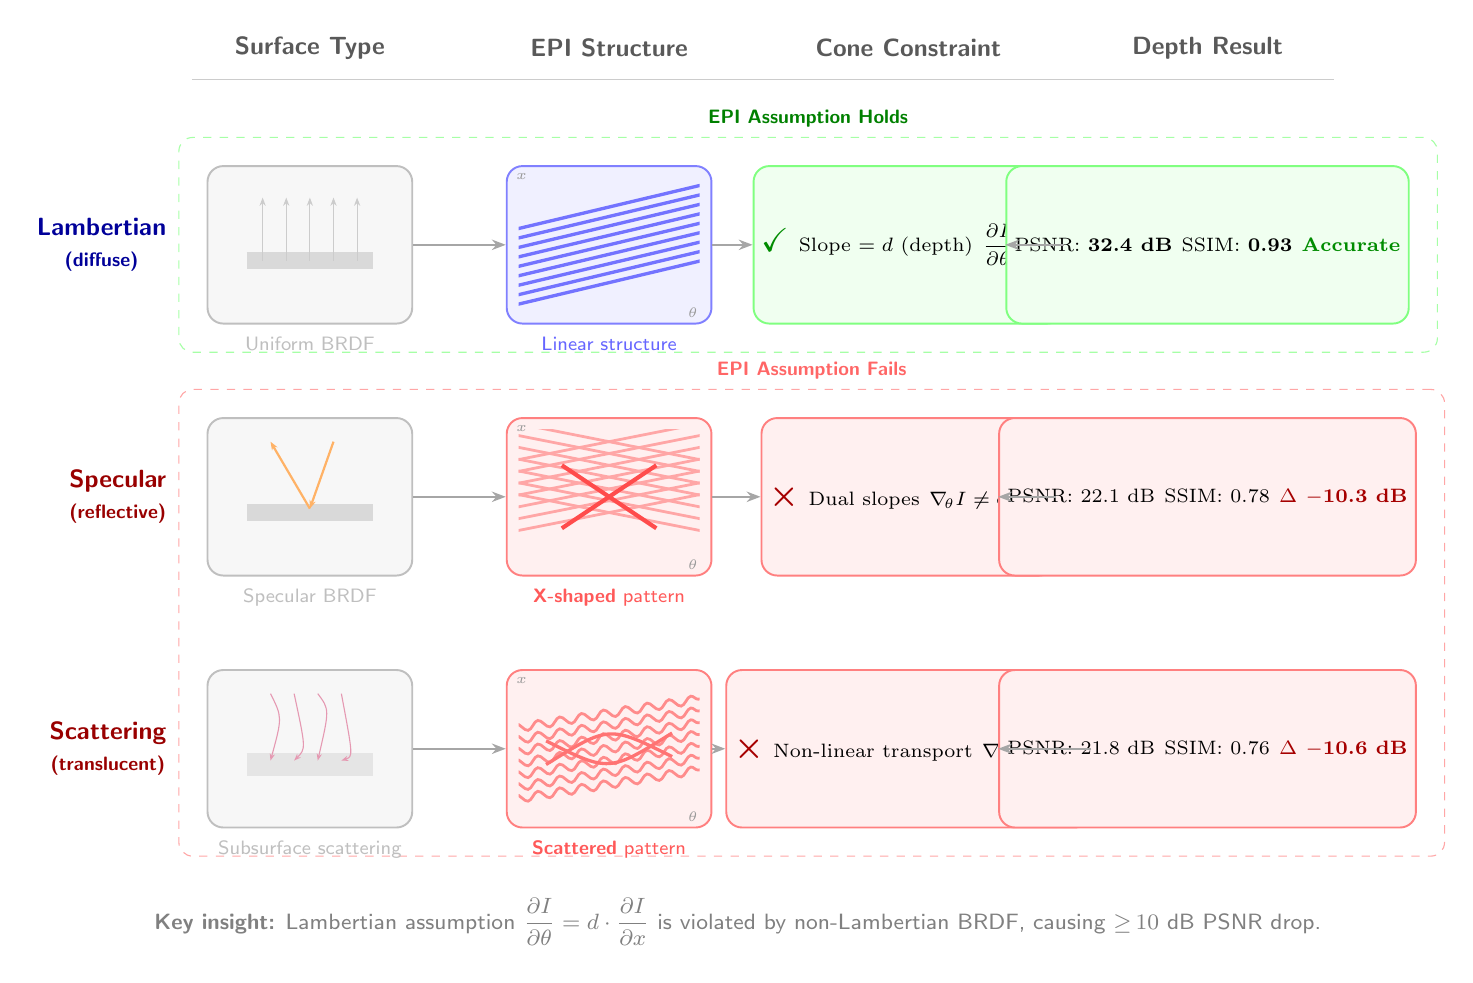
\begin{tikzpicture}[
    imgbox/.style={draw=#1!50, rounded corners=2mm, minimum width=2.6cm, minimum height=2.0cm,
                   inner sep=3pt, fill=#1!6, line width=0.7pt},
    colhead/.style={font=\sffamily\small\bfseries, text=black!65},
    rowlabel/.style={font=\sffamily\small\bfseries, text=#1!60!black, align=center},
    arr/.style={-{Stealth[length=5pt]}, thick, color=black!35},
    lbl/.style={font=\sffamily\scriptsize, text=black!50},
]

% Column headers
\node[colhead] at (0, 2.5) {Surface Type};
\node[colhead] at (3.8, 2.5) {EPI Structure};
\node[colhead] at (7.6, 2.5) {Cone Constraint};
\node[colhead] at (11.4, 2.5) {Depth Result};

% Separator line
\draw[black!20, line width=0.5pt] (-1.5, 2.1) -- (13.0, 2.1);

%% ============ ROW 1: LAMBERTIAN ============
\node[rowlabel=blue, left] at (-1.7, 0) {Lambertian\\{\scriptsize (diffuse)}};

% Surface box
\node[imgbox=gray] (s1) at (0, 0) {};
\draw[gray!30, line width=6pt] ($(s1.center)+(-0.8,-0.2)$) -- ($(s1.center)+(0.8,-0.2)$);
\foreach \x in {-0.6,-0.3,...,0.6} {
  \draw[-{Stealth[length=3pt]}, gray!40, thin] ($(s1.center)+(\x,-0.2)$) -- ($(s1.center)+(\x,0.6)$);
}
\node[font=\sffamily\scriptsize, text=gray!50, below=1pt] at (s1.south) {Uniform BRDF};

% EPI box - linear
\node[imgbox=blue] (e1) at (3.8, 0) {};
\begin{scope}
  \clip ($(e1.center)+(-1.15,-0.85)$) rectangle ($(e1.center)+(1.15,0.85)$);
  \foreach \i in {-4,-3,...,4} {
    \draw[blue!55, line width=1.2pt]
      ($(e1.west)+(0.05,{0.12*\i-0.3})$) -- ($(e1.east)+(-0.05,{0.12*\i+0.3})$);
  }
\end{scope}
\node[font=\tiny\sffamily, text=black!40] at ($(e1.south east)+(-0.25,0.15)$) {$\theta$};
\node[font=\tiny\sffamily, text=black!40] at ($(e1.north west)+(0.2,-0.15)$) {$x$};
\node[font=\sffamily\scriptsize, text=blue!60, below=1pt] at (e1.south) {Linear structure};

% Constraint box
\node[imgbox=green, minimum width=2.4cm] (c1) at (7.6, 0) {
  {\large\textcolor{green!55!black}{$\boldsymbol{\checkmark}$}}\\[6pt]
  {\scriptsize Slope $= d$ (depth)}\\[2pt]
  {\scriptsize $\dfrac{\partial I}{\partial\theta} \propto d$}
};

% Result box
\node[imgbox=green, minimum width=2.4cm] (r1) at (11.4, 0) {
  {\scriptsize PSNR: \textbf{32.4 dB}}\\[2pt]
  {\scriptsize SSIM: \textbf{0.93}}\\[6pt]
  {\scriptsize\textcolor{green!55!black}{\textbf{Accurate}}}
};

\draw[arr] (s1.east) -- (e1.west);
\draw[arr] (e1.east) -- (c1.west);
\draw[arr] (c1.east) -- (r1.west);

%% ============ ROW 2: SPECULAR ============
\node[rowlabel=red, left] at (-1.7, -3.2) {Specular\\{\scriptsize (reflective)}};

% Surface box
\node[imgbox=gray] (s2) at (0, -3.2) {};
\draw[gray!30, line width=6pt] ($(s2.center)+(-0.8,-0.2)$) -- ($(s2.center)+(0.8,-0.2)$);
\draw[-{Stealth[length=3pt]}, orange!60, thick] ($(s2.center)+(0.3,0.7)$) -- ($(s2.center)+(0.0,-0.15)$);
\draw[-{Stealth[length=3pt]}, orange!60, thick] ($(s2.center)+(0.0,-0.15)$) -- ($(s2.center)+(-0.5,0.7)$);
\node[font=\sffamily\scriptsize, text=gray!50, below=1pt] at (s2.south) {Specular BRDF};

% EPI box - X-shaped
\node[imgbox=red] (e2) at (3.8, -3.2) {};
\begin{scope}
  \clip ($(e2.center)+(-1.15,-0.85)$) rectangle ($(e2.center)+(1.15,0.85)$);
  \foreach \i in {-3,-2,...,3} {
    \draw[red!35, line width=1.0pt]
      ($(e2.west)+(0.05,{0.15*\i})$) -- ($(e2.east)+(-0.05,{0.15*\i+0.5})$);
  }
  \foreach \i in {-3,-2,...,3} {
    \draw[red!35, line width=1.0pt]
      ($(e2.west)+(0.05,{0.15*\i+0.5})$) -- ($(e2.east)+(-0.05,{0.15*\i})$);
  }
  \draw[red!70, line width=1.5pt] ($(e2.center)+(-0.6,-0.4)$) -- ($(e2.center)+(0.6,0.4)$);
  \draw[red!70, line width=1.5pt] ($(e2.center)+(-0.6,0.4)$) -- ($(e2.center)+(0.6,-0.4)$);
\end{scope}
\node[font=\tiny\sffamily, text=black!40] at ($(e2.south east)+(-0.25,0.15)$) {$\theta$};
\node[font=\tiny\sffamily, text=black!40] at ($(e2.north west)+(0.2,-0.15)$) {$x$};
\node[font=\sffamily\scriptsize, text=red!65, below=1pt] at (e2.south) {\textbf{X-shaped} pattern};

% Constraint box
\node[imgbox=red, minimum width=2.4cm] (c2) at (7.6, -3.2) {
  {\large\textcolor{red!65!black}{$\boldsymbol{\times}$}}\\[6pt]
  {\scriptsize Dual slopes}\\[2pt]
  {\scriptsize $\nabla_{\!\theta} I \neq \mathrm{const}$}
};

% Result box
\node[imgbox=red, minimum width=2.4cm] (r2) at (11.4, -3.2) {
  {\scriptsize PSNR: 22.1 dB}\\[2pt]
  {\scriptsize SSIM: 0.78}\\[6pt]
  {\scriptsize\textcolor{red!65!black}{\textbf{$\Delta$ $-$10.3 dB}}}
};

\draw[arr] (s2.east) -- (e2.west);
\draw[arr] (e2.east) -- (c2.west);
\draw[arr] (c2.east) -- (r2.west);

%% ============ ROW 3: SCATTERING ============
\node[rowlabel=red, left] at (-1.7, -6.4) {Scattering\\{\scriptsize (translucent)}};

% Surface box
\node[imgbox=gray] (s3) at (0, -6.4) {};
\draw[gray!20, line width=8pt] ($(s3.center)+(-0.8,-0.2)$) -- ($(s3.center)+(0.8,-0.2)$);
\foreach \x/\dy in {-0.5/0.3, -0.2/-0.1, 0.1/0.4, 0.4/-0.2} {
  \draw[-{Stealth[length=2.5pt]}, purple!40, thin]
    ($(s3.center)+(\x,0.7)$) .. controls ($(s3.center)+({\x+0.15},{\dy+0.1})$) .. ($(s3.center)+(\x,-0.15)$);
}
\node[font=\sffamily\scriptsize, text=gray!50, below=1pt] at (s3.south) {Subsurface scattering};

% EPI box - scattered
\node[imgbox=red] (e3) at (3.8, -6.4) {};
\begin{scope}
  \clip ($(e3.center)+(-1.15,-0.85)$) rectangle ($(e3.center)+(1.15,0.85)$);
  \foreach \i in {-3,-2,...,3} {
    \draw[red!45, line width=1.0pt, decorate, decoration={snake, amplitude=1.5pt, segment length=8pt}]
      ($(e3.west)+(0.05,{0.15*\i-0.2})$) -- ($(e3.east)+(-0.05,{0.15*\i+0.2})$);
  }
  \draw[red!55, line width=1.2pt] ($(e3.center)+(-0.8,0.1)$) .. controls ($(e3.center)+(0.0,-0.3)$) .. ($(e3.center)+(0.8,0.2)$);
  \draw[red!55, line width=1.2pt] ($(e3.center)+(-0.8,-0.2)$) .. controls ($(e3.center)+(0.0,0.3)$) .. ($(e3.center)+(0.8,-0.1)$);
\end{scope}
\node[font=\tiny\sffamily, text=black!40] at ($(e3.south east)+(-0.25,0.15)$) {$\theta$};
\node[font=\tiny\sffamily, text=black!40] at ($(e3.north west)+(0.2,-0.15)$) {$x$};
\node[font=\sffamily\scriptsize, text=red!65, below=1pt] at (e3.south) {\textbf{Scattered} pattern};

% Constraint box
\node[imgbox=red, minimum width=2.4cm] (c3) at (7.6, -6.4) {
  {\large\textcolor{red!65!black}{$\boldsymbol{\times}$}}\\[6pt]
  {\scriptsize Non-linear transport}\\[2pt]
  {\scriptsize $\nabla_{\!\theta} I$ varies}
};

% Result box
\node[imgbox=red, minimum width=2.4cm] (r3) at (11.4, -6.4) {
  {\scriptsize PSNR: 21.8 dB}\\[2pt]
  {\scriptsize SSIM: 0.76}\\[6pt]
  {\scriptsize\textcolor{red!65!black}{\textbf{$\Delta$ $-$10.6 dB}}}
};

\draw[arr] (s3.east) -- (e3.west);
\draw[arr] (e3.east) -- (c3.west);
\draw[arr] (c3.east) -- (r3.west);

% Grouping boxes
\begin{scope}[on background layer]
  \node[draw=green!35, dashed, rounded corners=5pt, inner sep=10pt,
        fit=(s1)(e1)(c1)(r1),
        label={[font=\sffamily\scriptsize\bfseries, text=green!50!black]above:EPI Assumption Holds}] {};
  \node[draw=red!35, dashed, rounded corners=5pt, inner sep=10pt,
        fit=(s2)(e2)(c2)(r2)(s3)(e3)(c3)(r3),
        label={[font=\sffamily\scriptsize\bfseries, text=red!60]above:EPI Assumption Fails}] {};
\end{scope}

% Bottom annotation
\node[font=\sffamily\footnotesize, text=black!50, align=center] at (5.5, -8.6) {
  \textbf{Key insight:} Lambertian assumption
  $\dfrac{\partial I}{\partial \theta} = d \cdot \dfrac{\partial I}{\partial x}$
  is violated by non-Lambertian BRDF, causing ${\geq}\,10$ dB PSNR drop.
};

\end{tikzpicture}
\end{document}